\section{Class M2: the minimum at a reverse centre and the nonshort cases}\label{sec:mixed}

A period of class $\cls{M2}$ has switches of both signs, every maximal reverse run has exactly two
switches, and some maximal forward run has at least two (\cref{def:classes}). Unlike the classes
$\cls{R}$, $\cls{F}$ and $\cls{M1}$, such a period has no rigid sign word: the forward runs may have
any lengths, the number of reverse runs is arbitrary, and the factors are unrelated. The exclusion
is therefore local. We look at a window of at most seven consecutive pieces around the smallest
active margin of the period, read the single normal multiplier $U$ of the whole period in that
window, and derive a finite list of scalar necessary conditions, which are then shown to be
inconsistent. The whole period enters only through three inputs: the compact domain
(\cref{thm:compact-domain}), the cap on the Casimir that competitiveness imposes, and a lower bound
on the Casimir obtained from the winding of the switch vectors over the period.

\begin{theorem}[Class $\cls{M2}$]\label{thm:class-M2}
Let $P$ be a competitive normal vertex period whose state stays in $\hstarstar$ and which has at
least six pieces. Then the sign sequence of $P$ is not of class $\cls{M2}$.
\end{theorem}

The proof has five steps.
\begin{enumerate}[label=(\arabic*)]
\item A global minimum of the active margins sits at the centre of a reverse run
(\cref{prop:m2-centre}).
\item Of the two turns beside that centre, choose the one with the smaller active margin; after
reflecting the period and reversing time if necessary, it follows the centre
(\cref{lem:m2-reflection}).
\item The switch after the chosen turn is forward or reverse. If it is reverse, the forward run
through the turn has a single switch (it is short), and \cref{sec:smaller-short} excludes the
window (\cref{thm:m2-smaller-short}). If it is forward, the run is nonshort, and the switch after
the next piece is again forward or reverse (\cref{prop:m2-window,prop:m2-continuation}).
\item A comparison that moves one margin to a boundary value turns the window into one scalar
residual $N$ that must be negative (\cref{lem:m2-comparison}), together with a short list of
necessary bounds (\cref{lem:m2-necessary}).
\item A reverse successor contradicts $N<0$ directly (\cref{thm:m2-reverse}). A forward successor
leaves a small region of parameters on which the Casimir of the period exceeds the competitive cap
(\cref{thm:m2-forward}).
\end{enumerate}
This section carries out steps (1), (2), (4), (5) and the nonshort half of (3). The polynomial
inequalities are collected in \cref{app:nonshort-estimates}. Throughout, $\gamma^2$ is the Casimir of
\cref{def:normal-multiplier}, and the switch norms and turn secants are those of
\cref{lem:switch-norms}.

\subsection{Three inputs from the whole period}\label{sec:m2-inputs}

The competitive cap of \cref{cor:casimir-cap} is not quite sharp enough for class $\cls{M2}$. We use
the spectral form of the cost--Casimir inequality \cite[\texttt{GLOBAL\_\allowbreak SPECTRAL\_\allowbreak COST\_\allowbreak CASIMIR}]{Notes}.

\begin{lemma}[Casimir bounds]\label{lem:m2-casimir}
Let $P$ be a normal vertex period with cost $\cost$ and primary costate $\Lambda_1$.
\begin{enumerate}[label=(\alph*)]
\item If $\det\Lambda_1(0)>0$ and $\Lambda_1(0)_{10}<0$, then
$\cost\ge\frac\pi3\bigl(\kappa+\frac32\bigr)$ with $\kappa=\sqrt{\det\Lambda_1(0)}$.
\item If $P$ is competitive, then $\gamma^2<9193/50000$.
\item If $P$ is competitive and mixed, then $\gamma^2>27/256$.
\end{enumerate}
\end{lemma}

\begin{proof}[Sketch]
(a) Write $\Lambda_1(0)=-\kappa\,hJh^{-1}$ and $B=h^{-1}g$. The maximum condition gives pointwise
$2\kappa m_s\le 3m_b$, where $m_b=-\frac12\tr(JX)$ is a third of the cost density and
$m_s=-\frac12\tr(JBXB^{-1})$. The argument $\theta$ of $(B_{00}+B_{11})+i(B_{10}-B_{01})$ has
$\theta'=(m_b+m_s)/(z+1)$ with $z=\frac12\norm{B}_F^2\ge1$, and $g(T)=R$ forces
$\Delta\theta\ge\pi/3$. The spectral inequality $(m_b+m_s)^2\le 4z\,m_bm_s$ combines these into the
bound, which is stronger than \cref{prop:cost-casimir} by the arithmetic--geometric mean inequality.
(b) Class $\cls{R}$ is impossible (\cref{thm:class-R}), so some switch is forward and has positive
norm; when $\gamma^2>0$, $\Lambda_1(0)$ is then negative elliptic (\cref{prop:ellipticity}), and
(a) with $\cost\le\Aoct<3.12606$ gives $\kappa<1.4853$, so $\gamma^2=\kappa^2/12<9193/50000$.
(c) If $\gamma^2\le 27/256$, the Gram identity (\cref{lem:gram}) with $d_\pm\ge3/32$ puts the angle
between consecutive switch vectors below $\pi/3$ at a forward piece, and above $2\pi/3$ at a reverse
centre, by the angle gap $\cos\varphi<3/10$ of \cref{sec:short-runs}; a turn
contributes nothing. The increments then add up to more than $\pi/3$, while the winding of the switch
vectors over one period is exactly $\pi/3$ (\cref{sec:short-runs}).
\end{proof}

At a reverse centre (the middle piece of a reverse run of two) the pairing and the Casimir are
explicit functions of four quantities. With active margin $a$, turn neighbours $p,n$ and incident
norms $u_{\mathrm i},u_{\mathrm o}$ (eight times the switch norms, which are turn secants), put
$r=a/(a+p)$, $t=a/(a+n)$ and $\rho=a^2/(a^2+4)$. Stationarity at the centre and the Gram identity
read
\begin{equation}\label{eq:m2-centre}
\gamma^2=\frac{4u_{\mathrm i}u_{\mathrm o}-E^2}{16(1-\rho)^2},\qquad
E=1+r+t-\rho+\log\frac{\rho}{rt}-\frac{1-u_{\mathrm i}}{r}-\frac{1-u_{\mathrm o}}{t}.
\end{equation}
The strict centre minimum gives $r,t<\frac12$, and the positive reverse factor gives $\rho<rt$.

\begin{lemma}[Scale of a reverse centre]\label{lem:m2-scale}
In a competitive mixed normal vertex period, every reverse centre has active margin $a$ with
$a^2<12/17$.
\end{lemma}

\begin{proof}
The bound is $\rho<3/20$. Lowering both incident norms to their common floor $3/4$, and then raising
both ratios $r,t$ to $\frac12$, only decreases the right side of \eqref{eq:m2-centre}, and gives
$\gamma^2>G(\rho)=(9/4-B(\rho)^2)/(16(1-\rho)^2)$ with $B(\rho)=1-\rho+\log(4\rho)$. The function
$G$ increases on $[3/20,1/4)$ and $G(3/20)>23/125>9193/50000$, which contradicts
\cref{lem:m2-casimir}(b) when $\rho\ge3/20$; and $\rho<rt<1/4$ always.
\Cref{fig:m2-domains}(a) shows $G$.
\end{proof}

\begin{figure}[tb]
\centering
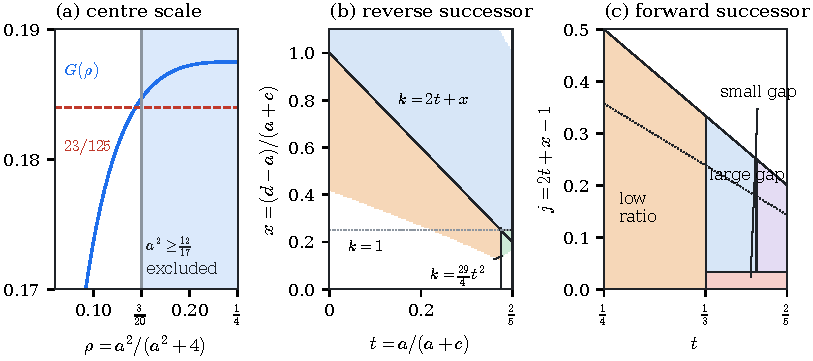
\includegraphics[width=\textwidth]{figures/fig-mixed-domains.pdf}
\caption{What the estimates of class $\cls{M2}$ control. (a)~The lower bound
$G(\rho)=(9/4-B(\rho)^2)/(16(1-\rho)^2)$ for the Casimir at a reverse centre, with
$\rho=a^2/(a^2+4)$. It exceeds the cap $23/125$ (dashed) on $[3/20,1/4)$, which proves
$a^2<12/17$ (\cref{lem:m2-scale}).
(b)~The parameters $(t,x)$ of the scalar reverse exclusion (\cref{prop:m2-reverse-core}), below
$x=1.1$, by the face to which $k$ is lowered: the unit shape $k=1$, the order face $k=2t+x$, and
the scale strip $k=29t^2/4$, which lies in $13/35<t<2/5$, $x\le9/35$. Points above $x=1$ belong to
the order face. (c)~The parameters $(t,j)$ of a forward successor, in $1/4<t<2/5$, $0<j<1-2t$: the
low ratio $t\le1/3$, the two large-gap regions $j\ge1/30$, split at $t=3/8$, and the small-gap
region, where the Casimir exceeds the cap. The dotted line is $j=\frac57(1-2t)$.}\label{fig:m2-domains}
\end{figure}

\subsection{The minimum is a reverse centre}\label{sec:m2-centre}

Let $a_m$ be a smallest active margin of the period; the active margins are periodic, so a minimum
exists. A minimum cannot be at a turn: at three pieces with labels $i,j,i$ the active margins are
strictly log-concave, $a_{k}a_{k+2}<a_{k+1}^2$ (\cref{lem:three-arc}), so the middle one is not the
smallest of the three. If both switches at $m$ are reverse, $m$ is the centre of a reverse run. The
remaining case, both switches forward, is excluded by the following theorem, which uses only
stationarity and the floors that the two missing controls impose.

\begin{proposition}[No small forward minimum]\label{prop:m2-small-forward}
Let $P$ be a normal vertex period with at least three pieces, and let $m$ be an index such that the
switches $m-2,m-1,m,m+1$ are forward, $a_m\le a_j$ for $m-2\le j\le m+2$, and $a_m^2\le4/3$. This is
impossible.
\end{proposition}

The proof \cite[\texttt{SMALL\_\allowbreak FORWARD\_\allowbreak MINIMUM\_\allowbreak HAND\_\allowbreak PROOF}]{Notes} writes the multiplier in the frame of
the central piece, eliminates one coordinate with stationarity at the centre, and keeps the
stationarity row at the smaller neighbour with the two exterior floors $v\ge F_x(q)$ at the forward
switches. The remaining face is a one-variable residual with an exactly controlled second
derivative; two integrations and the Pad\'e bound $\frac12(h-h^{-1})-\log h\ge (h-1)^3/(3h(h+1))$
leave a rational expression, negative by an elementary cubic comparison. No Casimir bound is used.

\begin{proposition}[The minimum is a reverse centre]\label{prop:m2-centre}
Let $P$ be a competitive normal vertex period of class $\cls{M2}$ with at least six pieces. There is
an index $m$ with $a_m\le a_k$ for every $k$ such that the switches $m-1$ and $m$ are reverse and the
switches $m-2$ and $m+1$ are forward.
\end{proposition}

\begin{proof}
Take a global minimum $m$. If exactly one of the switches $m-1,m$ is reverse, the pieces $m-1,m,m+1$
have labels $i,j,i$, and \cref{lem:three-arc} contradicts minimality. If both are forward, the
strict centre minimum of the neighbouring reverse runs (\cref{prop:run-structure}) forces the
switches $m-2$ and $m+1$ to be forward as well: otherwise the centre of the adjacent reverse run
would have a smaller active margin. The period is mixed, so it has a reverse centre; by
\cref{lem:m2-scale} its active margin squared is below $12/17$, hence $a_m^2<12/17<4/3$, and
\cref{prop:m2-small-forward} gives a contradiction. If both switches are reverse, they form a
maximal reverse run, of length two in class $\cls{M2}$, and $m$ is its centre.
\end{proof}

\subsection{Orientation by reflection}\label{sec:m2-reflection}

Let $S=\mathrm{diag}(1,-1)$. Reflecting the plane and reversing time is a symmetry of the control
problem: it maps a normal vertex period to another one with the same cost, and reverses the order of
the pieces.

\begin{lemma}[Reflection]\label{lem:m2-reflection}
For every normal vertex period $P$ there is a normal vertex period $P'$ with the same number of
pieces and the same cost, whose state stays in $\hstarstar$ when that of $P$ does, with labels
$i'_k=c-i_{-1-k}$ for a constant $c\in\Z/3$ and active margins $a'_k=a_{-1-k}$. Its switch $k$ is
forward if and only if the switch $-2-k$ of $P$ is forward, and $P'$ is of class $\cls{M2}$ when $P$
is.
\end{lemma}

The construction is $u'(t)=\varsigma u(T-t)$, with $\varsigma$ the permutation of the vertices that
reflects the labels, $g'(t)=SR^{-1}g(T-t)S$, $X'(t)=-SX(T-t)S$, and $\Lambda'(t)=-S\Lambda(T-t)S$ for
both costates. Since $SJS=-J$, the cost density is preserved, and $\hstarstar$ is symmetric under
$x\mapsto-x$. Reading the signs in reverse order does not negate them: a reverse switch of $P$
is a reverse switch of $P'$.

By \cref{prop:m2-centre,lem:m2-reflection} we may assume that the global minimum $a=a_m$ is a
reverse centre and that the turn after it is the smaller one: $a_{m+1}\le a_{m-1}$. (At a tie either
choice works.) After relabeling the vertices by a power of $R$, which changes neither the cost nor
the active margins, the pieces $m-2,\dots,m+3$ have labels and active margins
\begin{equation}\label{eq:m2-labels}
0(p),\quad 1(b),\quad 0(a),\quad 2(c),\quad 0(d),\quad 1(r)
\end{equation}
when the switch $m+2$ is forward.
These are consecutive pieces of the period, continued through the twisted seam when necessary; they
need not be distinct from other pieces named later, and they are not a closed competitor.

\subsection{The nonshort window}\label{sec:m2-window}

\begin{table}[t]
\centering\small
\begin{tabular}{@{}l>{\raggedright\arraybackslash}p{0.74\textwidth}@{}}
\toprule
Symbol & Meaning (in \cref{sec:mixed} and \cref{app:nonshort-estimates})\\
\midrule
$p,b,a,c,d,r$ & active margins of six consecutive pieces \eqref{eq:m2-labels}; $a$ is a global
minimum, and $c\le b$\\
$K_a,\ Q,\ K_r$ & $a^2+4$, $d^2+4$, $r^2+4$\\
$S,T,W,Z,Y$ & $a+b$, $a+c$, $c+d$, $d+r$, $W^2-T^2$ (here $T$ is not the terminal time)\\
$u,v,w$ & eight times the norms of the switches $b\to a$; $a\to c$ and $c\to d$; $d\to r$\\
$h_a,h_d$ & the diagonal entries of the multiplier in the frames of the pieces $a$ and $d$\\
$U(x),\ g_B(x)$ & $1-x+x^2$ and $(B^2+Bx+x^2)/(B+x)^2=1-Bx/(B+x)^2$\\
$\operatorname{Sec}(A,B,P)$ & the average of $g_B$ over the interval between $A$ and $P$\\
$F_x(q)$ & $1+x^2q-xq\log q/(q-1)$, with $F_x(1)=U(x)$\\
$t,x,k,q$ & $a/T$, $(d-a)/T$, $K_a/T^2$, $WZ/Q$ (normalized coordinates)\\
$j$ & $2t+x-1$, the gap of a forward successor\\
\bottomrule
\end{tabular}
\caption{Local notation of class $\cls{M2}$. The letters $p,r,t,u,x$ have their usual meaning
elsewhere in the paper.}\label{tab:m2-notation}
\end{table}

\Cref{tab:m2-notation} lists the local notation. All quantities in the window come from the one
normal multiplier of the period. The factors of the same-sign pieces follow from the one-arc map
(\cref{lem:one-arc}) and the margins $(a_k,a_{k+1},(4-a_ka_{k+1})/(a_k+a_{k+1}))$ of the state at a
switch: the factor of a piece with incident signs $++$, $--$, $-+$, $+-$ is $s_{k-1}s_k/K_k$,
$K_k/(s_{k-1}s_k)$, $s_k/s_{k-1}$, $s_{k-1}/s_k$ respectively. In the window this gives
the central factor $K_a/(ST)>1$, the factor $q=WZ/Q>1$ of the piece $d$, and $d>a$ from the turn
$c$.

Both switches at a turn have the same norm, the turn secant (\cref{lem:switch-norms}):
$u=\operatorname{Sec}(a,b,p)$ and $v=\operatorname{Sec}(a,c,d)$, where
\[
\operatorname{Sec}(A,B,P)=1+\frac{B^2}{(A+B)(P+B)}-\frac{B}{P-A}\log\frac{P+B}{A+B}.
\]
In the frame of the central piece the multiplier is
\begin{equation}\label{eq:m2-Ua}
U_a=\begin{pmatrix}h_a&-K_a^2v/(8S^2)\\ S^2u/8&-h_a\end{pmatrix},\qquad
\gamma^2=\det U_a=\frac{uvK_a^2}{64}-h_a^2,
\end{equation}
and stationarity at the centre (\cref{lem:stationarity}) fixes the diagonal:
\begin{equation}\label{eq:m2-ha}
\begin{gathered}
h_a=\frac{K_a}{16a}\bigl(Su+Tv-C(b,a,c)\bigr),\\
C(p,a,n)=p+a+n-\frac{a^2}{p+a}-\frac{a^2}{a+n}+\frac{a^3}{a^2+4}
-a\log\frac{(p+a)(a+n)}{a^2+4}.
\end{gathered}
\end{equation}
Here $C(p,a,n)$ is four times the partial derivative of the normalized cost $\cost/\sqrt{12}$ in
the active margin of a same-sign piece. Transport across the centre and the turn to the frame of
the piece $d$ gives
\begin{equation}\label{eq:m2-transport}
h_d=h_a+\frac{vY}{8},\qquad w=\frac{uK_a^2+16h_aY+vY^2}{Q^2},
\end{equation}
and stationarity at $d$, the first piece of the forward run after the turn, is the root equation
\begin{equation}\label{eq:m2-root}
R_d:=C(c,d,r)-Wv-Zw+\frac{16\,d\,h_d}{Q}=0.
\end{equation}

\begin{proposition}[The nonshort window]\label{prop:m2-window}
Let $P$ be competitive, with state in $\hstarstar$, of class $\cls{M2}$ and with at least six pieces;
let $m$ be as in \cref{prop:m2-centre} with $a_{m+1}\le a_{m-1}$, and let the switch $m+2$ be
forward. Then $(p,b,a,c,d,r)=(a_{m-2},\dots,a_{m+3})$, with $u,v,h_a,w$ as above, satisfy:
\begin{enumerate}[label=(\roman*)]
\item the order $a<b$, $a<c\le b$, $a<p$, $a<d$, $a\le r$;
\item strict star at the five switches, $pb,ab,ac,cd,dr<4$; the factors $ST<K_a$ and $Q<WZ$;
three-arc log-concavity $ad<c^2$;
\item the compact domain: $a\ge2/15$, $cd+\frac2{15}(c+d)\le4$, $dr+\frac2{15}(d+r)\le4$,
$d,r\le8$, and $a+c,\,c+d,\,d+r\ge\frac12$; and the scale bound $a^2<12/17$;
\item the turn secants $u=\operatorname{Sec}(a,b,p)$, $v=\operatorname{Sec}(a,c,d)$; the switching
inequalities $g_b(p)\le u\le g_b(a)$, $g_c(d)\le v\le g_c(a)$, $w\ge g_d(r)$; the missing-control
floors $v\ge F_{d/W}(q)$ and $w\ge F_{d/Z}(q)$;
\item the identities \eqref{eq:m2-ha}, \eqref{eq:m2-transport} and \eqref{eq:m2-root};
\item $27/256<uvK_a^2/64-h_a^2<9193/50000$.
\end{enumerate}
\end{proposition}

\begin{proof}[Sketch]
Each item is read off the costate cycle at the switches of the window: (i) from minimality, the
choice $c\le b$ and \cref{prop:run-structure}; (ii) from the margin transports (\cref{lem:one-arc});
(iii) from \cref{thm:compact-domain} at the switching times (every margin is at least $2/15$, and
$y\le9/2$ on $\hstarstar$ gives the pair sums and $d,r\le8$) and \cref{lem:m2-scale}; (iv) from
\cref{lem:switch-norms} and, for the floors, from $H_i\le0$ for the two controls missing at a forward
switch, written through stationarity
\cite[\texttt{MIXED\_\allowbreak GLOBAL\_\allowbreak SMALL\_\allowbreak FORWARD\_\allowbreak MINIMUM}~(11)--(12)]{Notes}, an identity algebraic in
$x$ that holds for every $x$; (v) from exact transports; (vi) from \cref{lem:m2-casimir}.
\end{proof}

\subsection{The successor of the forward piece}\label{sec:m2-continuation}

The window does not yet contain a contradiction: the root equation \eqref{eq:m2-root} has solutions
compatible with (i)--(vi). The next actual switch, after the piece $r$, supplies one more condition.
Finiteness of the representation guarantees that it exists, and equal neighbouring labels have
been merged, so it is forward or reverse. Let
\[
t_{\mathrm{next}}=\frac{Q^2v-16h_dZ^2+wZ^4}{K_r^2}
\]
be the norm of that switch when it is forward, read in the frame of the piece $r$.

\begin{proposition}[The continuation alternative]\label{prop:m2-continuation}
In the situation of \cref{prop:m2-window}:
\begin{enumerate}[label=(\alph*)]
\item if the switch $m+3$ is forward, to a piece with active margin $s$, then $s\ge a$, $rs<4$,
$K_r<Z(r+s)$, $t_{\mathrm{next}}\ge g_r(s)\ge\frac34$, and both missing-control floors hold at the
piece $r$;
\item if the switch $m+3$ is reverse, to a piece with active margin $A$, then $a\le A<d$, $Ad<r^2$,
$w=\operatorname{Sec}(A,r,d)$ and $w\le g_r(A)$.
\end{enumerate}
\end{proposition}

In (a) the inequality for $t_{\mathrm{next}}$ is the forward switching inequality at the piece $r$,
whatever the margin $s$ and the length of the forward run. In (b) the piece $r$ is a turn, both its
switches have the norm $\operatorname{Sec}(A,r,d)$, $A\ge a$ by minimality, and $Ad<r^2$ is
three-arc log-concavity. Since $g_r$ decreases on $(0,r)$ and $A<r$, extending the average from
$[A,d]$ to $[a,d]$ also gives $w\le\operatorname{Sec}(a,r,d)$; we use (b) as stated.

\subsection{The boundary comparison and the residual}\label{sec:m2-comparison}

The root equation \eqref{eq:m2-root} is affine in the incident norm $u$, with slope
\begin{equation}\label{eq:m2-Ru}
\partial_uR_d=\frac{K_a}{aQ^2}\bigl(dSQ-Z(aK_a+SY)\bigr)<0,
\end{equation}
negative because $Y>0$, $Z>Q/W$, and $dSQ-Z(aK_a+SY)<(Q/W)\{a(ST-K_a)+Sc(a-d)\}<0$. The reverse
switch $b\to a$ caps $u$ by the ceiling $U(a/S)=g_b(a)$, so the actual data satisfy
$R_d(U(a/S))\le R_d(u)=0$. Stationarity at $d$ thus asks for an incident norm that is not too large.
The obstruction we shall exhibit is that, on the necessary domain, it asks for a norm above the
ceiling.

Before testing this, we remove the margins $b$ and $p$. Keep $a,c,d,r$ and the actual $v$ fixed and
raise $b$ to $b_*=K_a/T-a$, the value at which the central factor $K_a/(ST)$ equals one. Write
$G(b)=R_d(U(a/(a+b));b)$ for the residual at the ceiling, with $h_a$ given by central stationarity at
the margin $b$.

\begin{lemma}[Boundary comparison]\label{lem:m2-comparison}
For the window of \cref{prop:m2-window}, $G(b_*)<0$; the root $u_*$ of $R_d(\,\cdot\,;b_*)=0$
satisfies $u_*<U(aT/K_a)$; and the outgoing norm $w_*$ of that boundary root satisfies $w_*<w$.
\end{lemma}

\begin{proof}
Along $[b,b_*]$ the derivative is $G'(b)=\partial_uR_d\cdot a(b-a)/(a+b)^3<0$, and at the actual
margin $G(b)=\partial_uR_d\,(U(a/S)-u)\le0$, so $G(b_*)<0$. Along the curve of roots $u(b)$, the
outgoing norm has $dw/db=dK_a^3G(b)/(aQ^3(\partial_uR_d)^2)<0$, so $w$ decreases from its actual
value.
\end{proof}

This is a scalar comparison: the point $b_*$ need not belong to a trajectory, and no switching
inequality, floor or Casimir bound is transported to it.

At $b_*$ the logarithm of the centre disappears ($C(b_*,a,c)=4/T+4c/K_a$), and homogeneity lets us
normalize by $T=a+c$. In the coordinates $t=a/T$, $x=(d-a)/T$, $k=K_a/T^2$, $q=WZ/Q$, write
$W=1+x$, $p=t+x$ and $B=k+2tx+x^2$ for the normalized values; the margins are recovered from
$(t,x,k,q)$, since $a^2(k-t^2)=4t^2$. The positive multiple
\[
N(t,x,k,q,v,\log q)=t\,B\,q\,W\cdot\frac{G(b_*)}{T}
\]
is a polynomial in $t,x,k,q,v$ and $L=\log q$, affine in $k$, in $v$ and in $L$; \cref{app:m2-residual} gives its coefficients. The normalized
incoming secant is $v=\operatorname{Sec}(t,1-t,t+x)=1+(1-t)^2/W-(1-t)\log W/x$.

\begin{lemma}[Shape monotonicity]\label{lem:m2-shape}
If $0<t<1$, $x>0$, $q\ge1$, $v\le U(t)$ and $L<q-1$, then $N(t,x,k,q,v,L)$ is nondecreasing in $k$.
\end{lemma}

The coefficient of $k$ is at least $q\,t\,x(1-t)\{(q-1)(2x+1)+tx\}>0$ (\cref{app:m2-residual}).
Since $k$ moves with $a$ at fixed $t$, the lemma lets every later argument lower $k$ to the smallest
value that the necessary conditions allow, and prove $N>0$ there.

\begin{lemma}[Necessary conditions]\label{lem:m2-necessary}
Every window of \cref{prop:m2-window} satisfies
\begin{enumerate}[label=(\roman*)]
\item $0<t<\frac12$, $x>0$, $k>1$, $1<q<W/p$, $v=\operatorname{Sec}(t,1-t,t+x)$,
$1-(1-t)p/W^2\le v\le U(t)$ and $F_{p/W}(q)\le v$;
\item $N(t,x,k,q,v,\log q)<0$;
\item $t<2/5$;
\item $a<4/5$, that is, $k>29t^2/4$;
\item $d^2+2cd>4$, that is, $k<2t+2x+x^2$;
\item $3d<7c$, that is, $x<\frac73-\frac{10}3t$;
\item if the successor is reverse, $d\le b_*$, that is, $k\ge2t+x$.
\end{enumerate}
\end{lemma}

Item (i) restates the window ($k>1$ is $ST<K_a$ with $S\ge T$, and $q<W/p$ is $dr<4$); the
others are proved in \cref{app:m2-bounds}.

\subsection{The reverse successor}\label{sec:m2-reverse}

\begin{proposition}[The scalar reverse exclusion]\label{prop:m2-reverse-core}
Let $0<t<2/5$, $x>0$, $\max\{1,\,2t+x,\,29t^2/4\}\le k<2t+2x+x^2$, $x<\frac73-\frac{10}3t$,
$1<q<(1+x)/(t+x)$, $v=\operatorname{Sec}(t,1-t,t+x)\le U(t)$ and $F_{(t+x)/(1+x)}(q)\le v$.
Then $N(t,x,k,q,v,\log q)>0$.
\end{proposition}

\begin{proof}
By \cref{lem:m2-shape} it suffices to find a shape $k'\le k$ allowed by the hypotheses with
$N(k')>0$. There are three exhaustive cases (\cref{fig:m2-domains}(b)).
\begin{enumerate}[label=(\arabic*)]
\item If $t\le13/35$ and $x\le1-2t$, lower $k$ to $1$, where $N(1)>0$ (\cref{lem:m2-unit-shape}).
\item If $2t+x\ge1$ and $x>1/4$, lower $k$ to the order face $k=2t+x$. The floor and the swapped
secant order give $q\le(1+x)/(2t+x)$. On this face $N$ is a positive
multiple of a function $\alpha+\beta q+\gamma/q-p\log q$, concave in $q$, so it suffices to check
$q=1$ and the upper end, where it is positive (\cref{lem:m2-order-face}).
\item Otherwise $13/35<t<2/5$ and $x\le9/35$; lower $k$ to the scale face $k=29t^2/4$, where
$N>0$ (\cref{lem:m2-strip}).\qedhere
\end{enumerate}
\end{proof}

On each face the logarithms are first replaced by rational bounds with the correct signs ($v$ by a
larger $\bar v$, $\log q$ by $L_+(q)\ge\log q$, the floor by a smaller $F_\ell$), which lowers $N$; the
result is a cubic in $y=q-1$ whose positivity for $y\ge0$ follows from six polynomial signs in
$(t,x)$. \Cref{app:m2-reverse-signs} gives the reduction and proves the signs.

\begin{theorem}[Reverse successor]\label{thm:m2-reverse}
No window of \cref{prop:m2-window} has a reverse successor.
\end{theorem}

\begin{proof}
By \cref{prop:m2-continuation}(b) and \cref{lem:m2-necessary}, the normalized window satisfies every
hypothesis of \cref{prop:m2-reverse-core}, which gives $N>0$, against \cref{lem:m2-necessary}(ii).
\end{proof}

\subsection{The forward successor}\label{sec:m2-forward}

When the successor is forward the order bound (vii) fails, and the residual alone does not suffice.
Two facts replace it. First, the scalar reverse exclusion applies to every window with $k\ge2t+x$,
without any assumption on the successor, so every window has the opposite order
\begin{equation}\label{eq:m2-order}
k<2t+x,\qquad\text{equivalently } d>b_*\text{ and } j=2t+x-1>0.
\end{equation}
Second, the forward successor gives a lower bound for the next norm at the
boundary root. Both the actual point and the boundary point satisfy the root equation
\eqref{eq:m2-root}, which makes $h_d$ an affine function of $w$; on that line the next norm is a
decreasing affine function of $w$, and $w_*<w$, so the next norm $t_{\mathrm{next},*}$ at the
boundary is at least $t_{\mathrm{next}}\ge\frac34$. As a function of the
incident norm the next norm is affine, and its value at the root differs from its value
$\mathcal T_U$ at the ceiling by a multiple of $N$. For multipliers $\alpha>0$ and $M\ge0$ the
combined residual
\begin{equation}\label{eq:m2-comb}
\begin{aligned}
\mathcal H&=\alpha N+C_*\bigl(\tfrac34-t_{\mathrm{next},*}\bigr)+M\bigl(F_{p/W}(q)-v\bigr)\\
&=(\alpha+1-Je^2)N+C_*\bigl(\tfrac34-\mathcal T_U\bigr)+M\bigl(F_{p/W}(q)-v\bigr),
\end{aligned}
\end{equation}
with $e=q/W$, $J=t+x(x+2)$ and an explicit $C_*>0$, is therefore negative at every window with a
forward successor. It is affine in $v$, in $\log q$ and in the floor value,
and a concave quadratic in $k$.

The unit face of the low-scale argument gives $t>1/4$ (\cref{lem:m2-low-unit}); with the
derivative floor $v\ge g_c(d)$ this gives $x<1$ and $4t+x<2$, and a quantitative form of the swapped
secant order gives $q<W/(1+2j)$. The remaining parameters are cut down in
three steps (\cref{fig:m2-domains}(c)).

\begin{proposition}[The forward successor in three steps]\label{prop:m2-forward-steps}
Every window of \cref{prop:m2-window} with a forward successor satisfies
\begin{enumerate}[label=(\alph*)]
\item $t>1/3$;
\item $j=2t+x-1<1/30$;
\end{enumerate}
and then the Casimir of the period is at least $9193/50000$, against \cref{lem:m2-casimir}(b).
\end{proposition}

\begin{proof}[Outline]
(a) If $t\le1/3$, take $\alpha=6$ and $M=0$. The coefficients of $v$ and of $\log q$ in $\mathcal H$
are negative, so raising $v$ to a rational majorant $\hat v$ and $\log q$ to $L_+(q)$ keeps
$\mathcal H$ negative. The result increases in $k$, so it is negative at $k=1$ as well; but at
$k=1$ it is positive (\cref{lem:m2-low-ratio}).

(b) Suppose $j\ge1/30$. Then $1/3<t<2/5$ by (a), and the derivative floor in integral form gives
$j<\frac57(1-2t)$. For $1/3\le t\le3/8$ take $\alpha=\frac72-10(q-1)$ and $M=8j+8(q-1)-\frac16$,
both positive here; after the substitutions of $v$, $\log q$ and the floor by rational bounds, the
residual increases in $k$ and is positive at $k=1$. For $3/8\le t<2/5$ take $\alpha=4$ and $M=1$;
the residual increases in $k$ and is positive at the scale face $k=29t^2/4$
(\cref{lem:m2-large-gap}).

(c) Now $1/3<t<2/5$, $0<j<1/30$ and $1\le k<31/30$. With $N<0$, a rational comparison in $q$ gives
$\chi=pq/W>4/7$ (\cref{lem:m2-chi}). On the stationarity line of the piece $d$, the diagonal $h_d$
is an affine function $H_d(w)$ of the outgoing norm, and the Casimir is
$\Gamma(w)=(4B^2vw-H_d(w)^2)/(16(k-t^2)^2)$ in normalized form. For
$w\ge3/4$ one has $\Gamma'(w)<0$ (\cref{lem:m2-slope}). The actual $w$ lies between $3/4$ and the
central upper envelope $w_U$, the transported norm with $u$ at its ceiling and $b=b_*$, so $\gamma^2=\Gamma(w)>\Gamma(w_U)$. At $w_U$ the event factor $q$ is
eliminated with the floor (\cref{lem:m2-qelim}), and the remaining function of $(t,x,k,v)$
exceeds $9193/50000$ (\cref{lem:m2-envelope}).
\end{proof}

\begin{theorem}[Forward successor]\label{thm:m2-forward}
No window of \cref{prop:m2-window} has a forward successor.
\end{theorem}

This is \cref{prop:m2-forward-steps}. The obstruction in its last step is the cost itself: the turn
data force the Casimir of the period above $9193/50000$, and by \cref{lem:m2-casimir}(a) a period
with such a Casimir costs more than $\Aoct$.

\begin{remark}[Small scale]\label{rem:m2-low-scale}
The same methods exclude every window with $a\le\frac12$, whatever the sign of the successor
\cite[\texttt{MIXED\_\allowbreak NONSHORT\_\allowbreak LOW\_\allowbreak SCALE\_\allowbreak HAND\_\allowbreak EXCLUSION}]{Notes}: then $k\ge17t^2$, and
$N$ can be lowered to $k=1$ or to $k=2t+\frac12$. The proof above needs only the unit face of that
argument (\cref{lem:m2-low-unit}), which gives $t>1/4$.
\end{remark}


\subsection{Proof of \texorpdfstring{\cref{thm:class-M2}}{the theorem for class M2}}\label{sec:m2-proof}

Let $P$ be as in \cref{thm:class-M2}, and take $m$ from \cref{prop:m2-centre}. If $a_{m+1}>a_{m-1}$,
replace $P$ by its reflection (\cref{lem:m2-reflection}): it is again competitive, of class
$\cls{M2}$, with state in $\hstarstar$ and the same number of pieces; the minimum moves to $-1-m$,
the four switches around it keep their signs in reverse order, and the smaller turn now follows the
centre. If the switch $m+2$ after the turn is reverse, the seven pieces $m-2,\dots,m+4$ form a
smaller-short window, excluded by \cref{thm:m2-smaller-short}. If it is forward, \cref{prop:m2-window} gives a nonshort window,
and \cref{prop:m2-continuation} gives a forward or a reverse successor; \cref{thm:m2-forward}
and \cref{thm:m2-reverse} exclude them. \qed
